\documentclass[]{report}
\usepackage{kotex}
\usepackage{verbatim} 
\usepackage{graphicx} 

\usepackage{listings}
\usepackage{color}

\definecolor{dkgreen}{rgb}{0,0.6,0}
\definecolor{gray}{rgb}{0.5,0.5,0.5}
\definecolor{mauve}{rgb}{0.58,0,0.82}

\lstset{frame=tb,
	language=Python,
	aboveskip=3mm,
	belowskip=3mm,
	showstringspaces=false,
	columns=flexible,
	basicstyle={\small\ttfamily},
	numbers=none,
	numberstyle=\tiny\color{gray},
	keywordstyle=\color{blue},
	commentstyle=\color{dkgreen},
	stringstyle=\color{mauve},
	breaklines=true,
	breakatwhitespace=true,
	tabsize=3
}


% Title Page
\title{HW04 - REPORT}
\author{정보컴퓨터공학부 201624536 이국현}


\begin{document}
\maketitle
\chapter{서론}

\begin{itemize}
	\item Corner Detection
	\item Feature Descriptor (SIFT)
	\item Feature Matching
	% \item Alignment
	\item RANSAC\\
\end{itemize}

HW04는 두 이미지에서 같은 Object를 인식하여 매칭하는 것이 목적이다. 이를 위해 위와 같이 4 단계의 작업이 수행된다.\\

\section{Corner Detection}

첫 번째 단계로 이미지의 Feature를 찾아내기 위해서 Harris operator를 사용할 수 있다.\\


\section{Feature Descriptor (SIFT)}

Feature를 판단할 때 단순히 한 point를 고려하는 것이 아니라, 주변의 Pixel들까지 반영하기 위해,
효과적으로 Descriptor를 비교할 수 있는 SIFT (Scale Invariant Feature Transform)을 이용할 수 있다.\\

\begin{figure}[ht!]
	\centering
	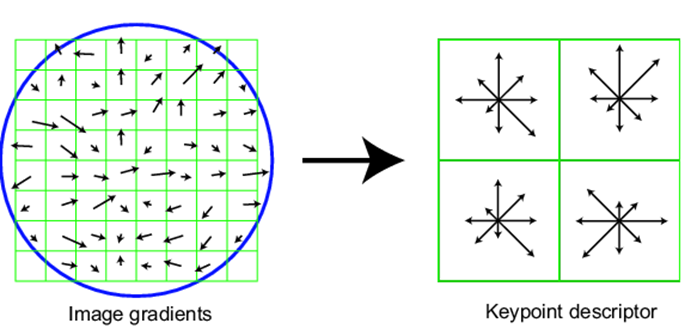
\includegraphics[width=0.9\textwidth]{image/1-2-SIFT.png}
	\caption{SIFT}
	\label{1-2}
\end{figure}

\section{Feature Matching}

두 이미지에서 연관된 Feature를 매칭하기 위해 SIFT로 구한 두 이미지의 모든 Descriptor vector에 대해서 Angle을 계산하고 Angle이 작은 Match를 선택한다.\

\[ angle = \arccos(\vec{des1} \cdot \vec{des2}) \]

Image1과 Image2의 모든 Feature에 대해서 서로 간의 Distance를 구하고 Distance가 가장 작은 것 끼리 매칭한다.
 이때, Best match와 Second match의 Distance에 큰 차이가 없다면 해당 Match는 선택하지 않는다.\\

 \[ ratio =  angleBest / angleSecond \]
 
 두 Distance를 비교하는 기준으로 Angle ratio를 사용한다. Angle ratio가 Threshold보다 작을때 Match를 선택한다.\\

% \section{Alignment}
\section{RANSAC}

Feature matching을 완벽하게 수행한다고 보장할 수는 없다. 매칭된 일부 Feature Pair들은 전혀 관련이 없는 Feature일 수 있다. 
이를 Outlier라고 하며, 이 Outlier를 제거하기 위해 RANSAC을 사용할 수 있다. RANSAC의 단계는 다음과 같다.\\

\begin{enumerate}
	\item Matched pairs에서 랜덤으로 Match를 Model로 선택
	\item 각 Model에서 Transformation 구한다 (Scaling, Rotation)
	\item Transformation을 비교해 Inlier 개수 세기
	\item 1. ~ 3.을 10번 반복
	\item Inlier가 가장 많은 Model 선택
	\item 해당 Model에서 Outlier를 제거한다.\\
\end{enumerate}

\chapter{본론}

\section{Prob 1: FindBestmatches}

\begin{lstlisting}

def FindBestMatches(descriptors1, descriptors2, threshold):
    assert isinstance(descriptors1, np.ndarray)
    assert isinstance(descriptors2, np.ndarray)
    assert isinstance(threshold, float)
    ## START
    ## the following is just a placeholder to show you the output format
    matched_pairs = []
    # dot 연산을 통해 descriptor1의 각 벡터와 descriptor 2의 벡터에 대해서 모두 내적한 행렬을 생성한다.
    # 모든 element에 arc cosine를 적용해 angle을 생성한다.
    angleTable = np.arccos(np.dot(descriptors1, descriptors2.T))
    for index1, angleArray in enumerate(angleTable):
        # vector1과 angle이 가장 작은 vector2를 찾는다.
        sortedAngleArray = list(enumerate(angleArray))
        sortedAngleArray.sort(key=lambda t:t[1])
        matchSt = sortedAngleArray[0]
        matchNd = sortedAngleArray[1]
        # best match와 second match의 angle ratio가 threshold보다 작을 때만 선택한다.
        ratio = np.abs(matchSt[1] / matchNd[1])
        if(ratio <= threshold):
            matched_pairs.append([index1, matchSt[0]])
    ## END
    return matched_pairs

\end{lstlisting}

Image1의 모든 Descriptor vector와 Image2의 모든 Descriptor vector에 대해서 내적하기 위해
두 2차원 행렬에 dot 연산을 하였다. 그리고 각 행에 대해서 가장 Angle이 낮은 Match를 선택하였다.
이때 Best match와 Second match의 Angle ratio가 Threshold보다 낮을 때만 선택하도록 구현하였다.\\

\section{Prob 2: RANSAC}

\begin{lstlisting}
def getTranform(feat1, feat2):
    tScaling = feat1[2] / feat2[2]
    tRotation = feat1[3] - feat2[3]
    tRotation = (tRotation + 2 * np.pi) % (2 * np.pi)  # delete negative
    tRotation = tRotation * 180 / np.pi                # radian to degree
    return tScaling, tRotation

def checkRange(tScaling, tRotation, tScalingComp, tRotationComp, orient_agreement, scale_agreement):
    tScaleRange = tScaling * scale_agreement
    if(np.abs(tScaling - tScalingComp) < tScaleRange):
        if(np.abs(tRotation - tRotationComp) < orient_agreement or np.abs(tRotation - tRotationComp) > 360 - orient_agreement):
            return True
    return False

def RANSACFilter(
        matched_pairs, keypoints1, keypoints2,
        orient_agreement, scale_agreement):

    assert isinstance(matched_pairs, list)
    assert isinstance(keypoints1, np.ndarray)
    assert isinstance(keypoints2, np.ndarray)
    assert isinstance(orient_agreement, float)
    assert isinstance(scale_agreement, float)
    ## START
    maxCount = 0
    maxIndex = 0
    for k in range(10):
        # matched_pairs에서 랜덤으로 match 선택
        i = random.randint(0, len(matched_pairs) - 1)
        (index1, index2) = matched_pairs[i]
        # match에서 transformation을 구한다 (scaling, rotation)
        tScaling, tRotation = getTranform(keypoints1[index1], keypoints2[index2])
        inlierCount = 0
        # 다른 모든 match를 다시 순회하면서 inlier counting
        for comp1, comp2 in matched_pairs:
            if(comp1 == index1 and comp2 == index2):
                continue
            tScalingComp, tRotationComp = getTranform(keypoints1[comp1], keypoints2[comp2])
            if(checkRange(tScaling, tRotation, tScalingComp, tRotationComp, orient_agreement, scale_agreement)):
                inlierCount += 1
        # inlier가 가장 많은 match 선택
        if(inlierCount > maxCount):
            maxCount = inlierCount
            maxIndex = i
    
    # 선택된 match에서 동일한 방식으로 inlier만 추출하여 return
    index1, index2 = matched_pairs[maxIndex]
    largest_set = [matched_pairs[maxIndex]]
    tScaling, tRotation = getTranform(keypoints1[index1], keypoints2[index2])
    inlierCount = 0
    for comp1, comp2 in matched_pairs:
        if(comp1 == index1 and comp2 == index2):
            continue
        tScalingComp, tRotationComp = getTranform(keypoints1[comp1], keypoints2[comp2])
        if(checkRange(tScaling, tRotation, tScalingComp, tRotationComp, orient_agreement, scale_agreement)):
            largest_set.append([comp1, comp2])
    print(len(largest_set), '/', len(matched_pairs))
    
    ## END
    assert isinstance(largest_set, list)
    return largest_set
\end{lstlisting}

matched\_pairs에서 랜덤으로 Match를 10번 선택하여,
각 Match와 다른 모든 Match에 대해서 Scale transform, Rotation transform의 차이를 비교하여 Inlier/Outlier를 판단한다.
랜덤으로 선택한 10개의 Match 중에 Inlier가 가장 많은 Match를 Model로 선택하고, 해당 Model에서 Outlier를 제거하여 return한다.\\


\chapter{결론}

\section{FindBestmatches}

\begin{figure}[ht!]
	\centering
	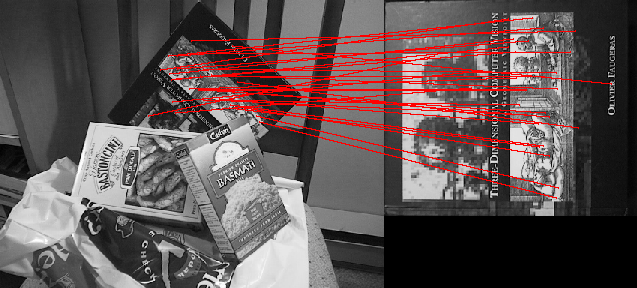
\includegraphics[width=0.7\textwidth]{image/3-1-book.png}
	\caption{Book}
	\label{3-1-book}
\end{figure}

Scene - Book에서는 FindBestmatches의 threshold=0.58일 때 31개의 Inlier와 0개의 Outlier로
가장 적은 Outlier를 가지면서 가장 많은 Inlier를 가지는 지점이다. 따라서 0.58을 적절한 Threshold로 설정하였다.\\

\begin{figure}[ht!]
	\centering
	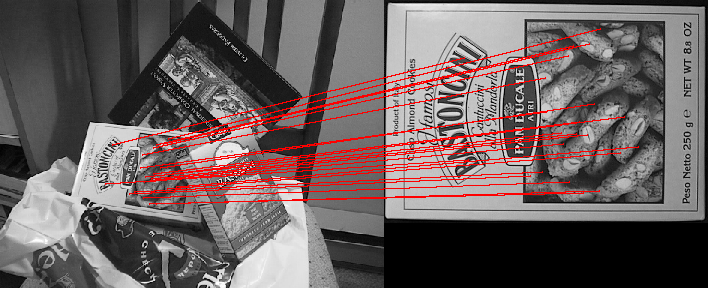
\includegraphics[width=0.7\textwidth]{image/3-1-box.png}
	\caption{Box}
	\label{3-1-box}
\end{figure}

Scene - Book에서는 FindBestmatches의 threshold=0.52일 때 26개의 Inlier와 0개의 Outlier로
가장 적은 Outlier를 가지면서 가장 많은 Inlier를 가지는 지점이다. 따라서 0.52를 적절한 Threshold로 설정하였다.\\

\section{RANSAC}

\begin{figure}[ht!]
	\centering
	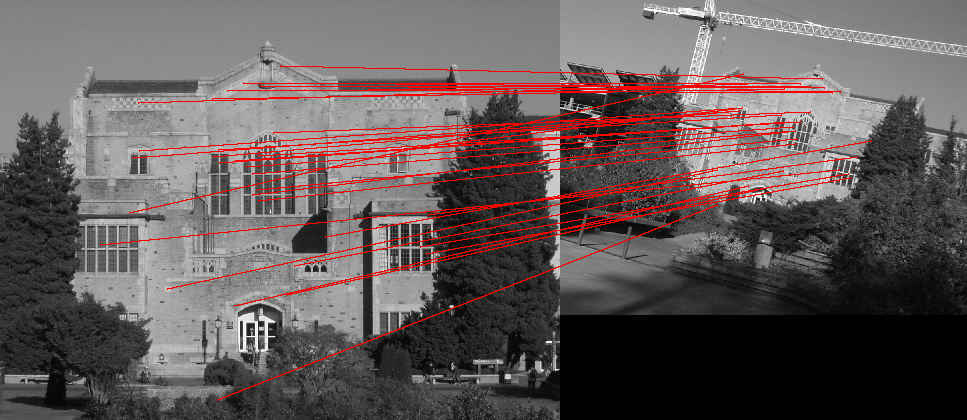
\includegraphics[width=0.9\textwidth]{image/3-2-library.png}
	\caption{Library}
	\label{3-2-library}
\end{figure}

RANSAC Filter를 테스트할 수 있도록 FindBestmatches에서 threshold=0.65로 설정하였다. 
이때 36개의 Match가 생기지만 몇 가지 적절하지 않은 Feature matching을 확인할 수 있다.\\

\begin{figure}[ht!]
	\centering
	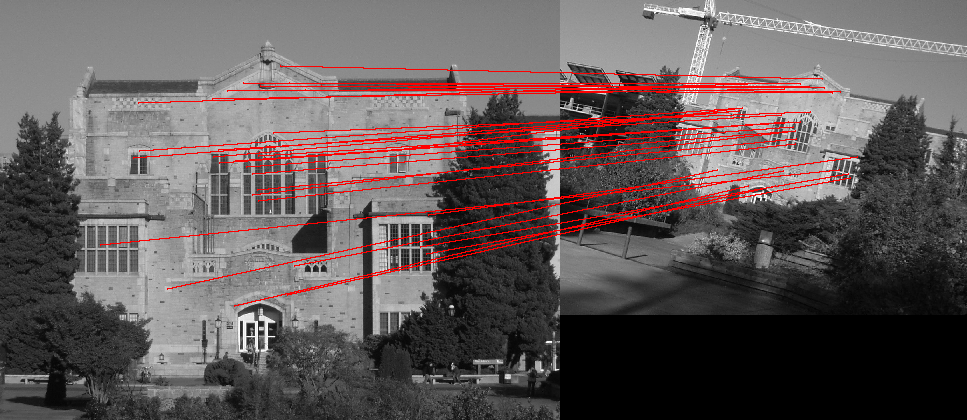
\includegraphics[width=0.9\textwidth]{image/3-2-libraryF.png}
	\caption{Library}
	\label{3-2-libraryF}
\end{figure}

RANSAC Filter에서 orient\_agreement=30, scale\_agreement=0.25로 설정하였을 때,
이미지에서 확인할 수 있는 Inlier를 제거하지 않으면서 3개의 Outlier를 제거할 수 있었다.

\end{document}          
